% Options for packages loaded elsewhere
\PassOptionsToPackage{unicode}{hyperref}
\PassOptionsToPackage{hyphens}{url}
%
\documentclass[
  ignorenonframetext,
]{beamer}
\usepackage{pgfpages}
\setbeamertemplate{caption}[numbered]
\setbeamertemplate{caption label separator}{: }
\setbeamercolor{caption name}{fg=normal text.fg}
\beamertemplatenavigationsymbolsempty
% Prevent slide breaks in the middle of a paragraph
\widowpenalties 1 10000
\raggedbottom
\setbeamertemplate{part page}{
  \centering
  \begin{beamercolorbox}[sep=16pt,center]{part title}
    \usebeamerfont{part title}\insertpart\par
  \end{beamercolorbox}
}
\setbeamertemplate{section page}{
  \centering
  \begin{beamercolorbox}[sep=12pt,center]{part title}
    \usebeamerfont{section title}\insertsection\par
  \end{beamercolorbox}
}
\setbeamertemplate{subsection page}{
  \centering
  \begin{beamercolorbox}[sep=8pt,center]{part title}
    \usebeamerfont{subsection title}\insertsubsection\par
  \end{beamercolorbox}
}
\AtBeginPart{
  \frame{\partpage}
}
\AtBeginSection{
  \ifbibliography
  \else
    \frame{\sectionpage}
  \fi
}
\AtBeginSubsection{
  \frame{\subsectionpage}
}

\usepackage{amsmath,amssymb}
\usepackage{lmodern}
\usepackage{iftex}
\ifPDFTeX
  \usepackage[T1]{fontenc}
  \usepackage[utf8]{inputenc}
  \usepackage{textcomp} % provide euro and other symbols
\else % if luatex or xetex
  \usepackage{unicode-math}
  \defaultfontfeatures{Scale=MatchLowercase}
  \defaultfontfeatures[\rmfamily]{Ligatures=TeX,Scale=1}
\fi
% Use upquote if available, for straight quotes in verbatim environments
\IfFileExists{upquote.sty}{\usepackage{upquote}}{}
\IfFileExists{microtype.sty}{% use microtype if available
  \usepackage[]{microtype}
  \UseMicrotypeSet[protrusion]{basicmath} % disable protrusion for tt fonts
}{}
\makeatletter
\@ifundefined{KOMAClassName}{% if non-KOMA class
  \IfFileExists{parskip.sty}{%
    \usepackage{parskip}
  }{% else
    \setlength{\parindent}{0pt}
    \setlength{\parskip}{6pt plus 2pt minus 1pt}}
}{% if KOMA class
  \KOMAoptions{parskip=half}}
\makeatother
\usepackage{xcolor}
\newif\ifbibliography
\setlength{\emergencystretch}{3em} % prevent overfull lines
\setcounter{secnumdepth}{-\maxdimen} % remove section numbering


\providecommand{\tightlist}{%
  \setlength{\itemsep}{0pt}\setlength{\parskip}{0pt}}\usepackage{longtable,booktabs,array}
\usepackage{calc} % for calculating minipage widths
\usepackage{caption}
% Make caption package work with longtable
\makeatletter
\def\fnum@table{\tablename~\thetable}
\makeatother
\usepackage{graphicx}
\makeatletter
\def\maxwidth{\ifdim\Gin@nat@width>\linewidth\linewidth\else\Gin@nat@width\fi}
\def\maxheight{\ifdim\Gin@nat@height>\textheight\textheight\else\Gin@nat@height\fi}
\makeatother
% Scale images if necessary, so that they will not overflow the page
% margins by default, and it is still possible to overwrite the defaults
% using explicit options in \includegraphics[width, height, ...]{}
\setkeys{Gin}{width=\maxwidth,height=\maxheight,keepaspectratio}
% Set default figure placement to htbp
\makeatletter
\def\fps@figure{htbp}
\makeatother

\makeatletter
\makeatother
\makeatletter
\makeatother
\makeatletter
\@ifpackageloaded{caption}{}{\usepackage{caption}}
\AtBeginDocument{%
\ifdefined\contentsname
  \renewcommand*\contentsname{Table of contents}
\else
  \newcommand\contentsname{Table of contents}
\fi
\ifdefined\listfigurename
  \renewcommand*\listfigurename{List of Figures}
\else
  \newcommand\listfigurename{List of Figures}
\fi
\ifdefined\listtablename
  \renewcommand*\listtablename{List of Tables}
\else
  \newcommand\listtablename{List of Tables}
\fi
\ifdefined\figurename
  \renewcommand*\figurename{Figure}
\else
  \newcommand\figurename{Figure}
\fi
\ifdefined\tablename
  \renewcommand*\tablename{Table}
\else
  \newcommand\tablename{Table}
\fi
}
\@ifpackageloaded{float}{}{\usepackage{float}}
\floatstyle{ruled}
\@ifundefined{c@chapter}{\newfloat{codelisting}{h}{lop}}{\newfloat{codelisting}{h}{lop}[chapter]}
\floatname{codelisting}{Listing}
\newcommand*\listoflistings{\listof{codelisting}{List of Listings}}
\makeatother
\makeatletter
\@ifpackageloaded{caption}{}{\usepackage{caption}}
\@ifpackageloaded{subcaption}{}{\usepackage{subcaption}}
\makeatother
\makeatletter
\@ifpackageloaded{tcolorbox}{}{\usepackage[many]{tcolorbox}}
\makeatother
\makeatletter
\@ifundefined{shadecolor}{\definecolor{shadecolor}{rgb}{.97, .97, .97}}
\makeatother
\makeatletter
\makeatother
\ifLuaTeX
  \usepackage{selnolig}  % disable illegal ligatures
\fi
\IfFileExists{bookmark.sty}{\usepackage{bookmark}}{\usepackage{hyperref}}
\IfFileExists{xurl.sty}{\usepackage{xurl}}{} % add URL line breaks if available
\urlstyle{same} % disable monospaced font for URLs
\hypersetup{
  pdftitle={Synthetic data generation with mice},
  hidelinks,
  pdfcreator={LaTeX via pandoc}}

\title{Synthetic data generation with \texttt{mice}}
\author{}
\date{}

\begin{document}
\frame{\titlepage}
\ifdefined\Shaded\renewenvironment{Shaded}{\begin{tcolorbox}[boxrule=0pt, borderline west={3pt}{0pt}{shadecolor}, enhanced, sharp corners, frame hidden, breakable, interior hidden]}{\end{tcolorbox}}\fi

\begin{frame}
\end{frame}

\begin{frame}{Disclaimer}
\protect\hypertarget{disclaimer}{}
I owe a debt of gratitude to many people as the thoughts and teachings
in my slides are the process of years-long development cycles and
discussions with my team, friends, colleagues and peers. When someone
has contributed to the content of the slides, I have credited their
authorship.

When external figures and other sources are shown:

\begin{enumerate}
[1)]
\tightlist
\item
  the references are included when the origin is known, or
\item
  the objects are directly linked from within the public domain and the
  source can be obtained by right-clicking the objects.
\end{enumerate}

Opinions are my own.
\end{frame}

\begin{frame}{This meeting}
\protect\hypertarget{this-meeting}{}
\begin{enumerate}
\tightlist
\item
  In retrospect.
\item
  What to do with uncertainty without a truth?
\item
  Some reasoning when you know you're wrong.
\end{enumerate}
\end{frame}

\begin{frame}{Terms I may use}
\protect\hypertarget{terms-i-may-use}{}
\begin{itemize}
\tightlist
\item
  TDGM: True data generating model
\item
  DGP: Data generating process, closely related to the TDGM, but with
  all the wacky additional uncertainty
\item
  Truth: The comparative truth that we are interested in
\item
  Bias: The distance to the comparative truth
\item
  Variance: When not everything is the same
\item
  Estimate: Something that we calculate or guess
\item
  Estimand: The thing we aim to estimate and guess
\item
  Population: That larger entity without sampling variance
\item
  Sample: The smaller thing with sampling variance
\item
  Incomplete: There exists a more complete version, but we don't have it
\item
  Observed: What we have
\item
  Unobserved: What we would also like to have
\end{itemize}
\end{frame}

\hypertarget{in-retrospect}{%
\section{In retrospect}\label{in-retrospect}}

\begin{frame}{At the start}
\protect\hypertarget{at-the-start}{}
We began this course series with a lecture on statistical inference.

Statistical inference is the process of drawing conclusions from truths

Truths are boring, but they are convenient.

\begin{itemize}
\tightlist
\item
  however, for most problems truths require a lot of calculations,
  tallying or a complete census.
\item
  therefore, a proxy of the truth is in most cases sufficient
\item
  An example for such a proxy is a \textbf{sample}
\item
  Samples are widely used and have been for a long timeSee
  \href{https://www.google.com/url?sa=t\&rct=j\&q=\&esrc=s\&source=web\&cd=\&ved=2ahUKEwjkyPTCs4L3AhUCuKQKHUpmBvIQFnoECAMQAw\&url=https\%3A\%2F\%2Fwww.cbs.nl\%2F-\%2Fmedia\%2Fimported\%2Fdocuments\%2F2009\%2F07\%2F2009-15-x10-pub.pdf\&usg=AOvVaw3BpUW2s_k0MB5yH1o-QGf2}{Jelke
  Bethlehem's CBS discussion paper} for an overview of the history of
  sampling within survey statistics
\end{itemize}
\end{frame}

\begin{frame}{Being wrong about the truth}
\protect\hypertarget{being-wrong-about-the-truth}{}
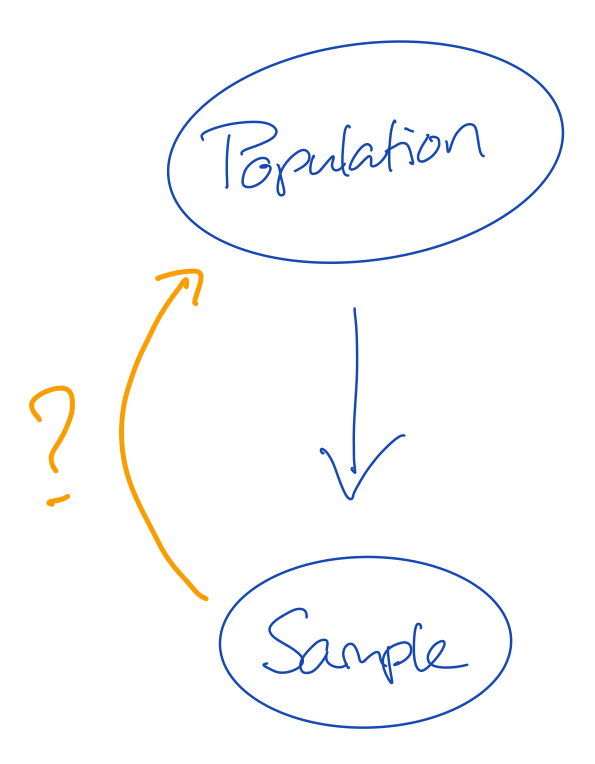
\includegraphics[width=0.9\textwidth,height=\textheight]{img/2. missingness_problem.png}

\begin{itemize}
\tightlist
\item
  The population is the truth
\item
  The sample comes from the population, but is generally smaller in size
\item
  This means that not all cases from the population can be in our sample
\item
  If not all information from the population is in the sample, then our
  sample may be \emph{wrong} Q1: Why is it important that our sample is
  not wrong? Q2: How do we know that our sample is not wrong?
\end{itemize}
\end{frame}

\begin{frame}{Solving the missingness problem}
\protect\hypertarget{solving-the-missingness-problem}{}
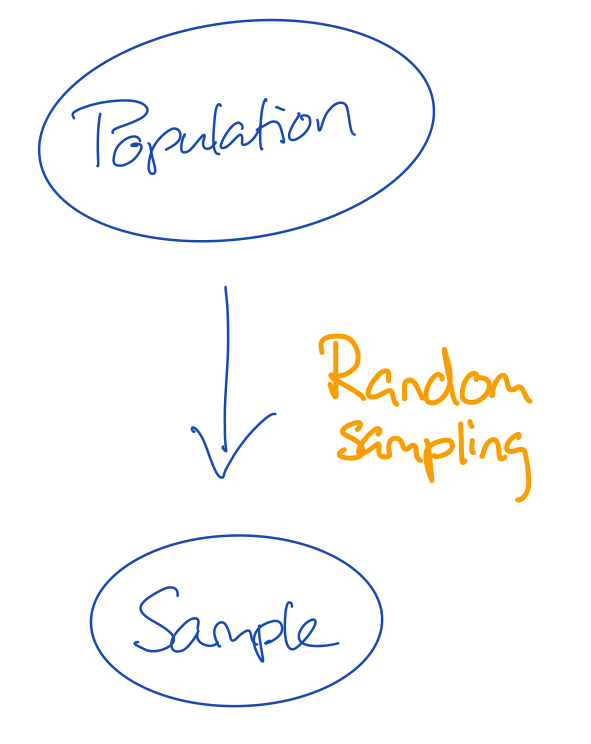
\includegraphics[width=0.9\textwidth,height=\textheight]{img/3. random_sampling.png}

\begin{itemize}
\tightlist
\item
  There are many flavours of sampling
\item
  If we give every unit in the population the same probability to be
  sampled, we do \textbf{random sampling}
\item
  The convenience with random sampling is that the missingness problem
  can be ignored
\item
  The missingness problem would in this case be: \textbf{not every unit
  in the population has been observed in the sample}
\end{itemize}

Q3: Would that mean that if we simply observe every potential unit, we
would be unbiased about the truth?
\end{frame}

\begin{frame}{Sidestep}
\protect\hypertarget{sidestep}{}
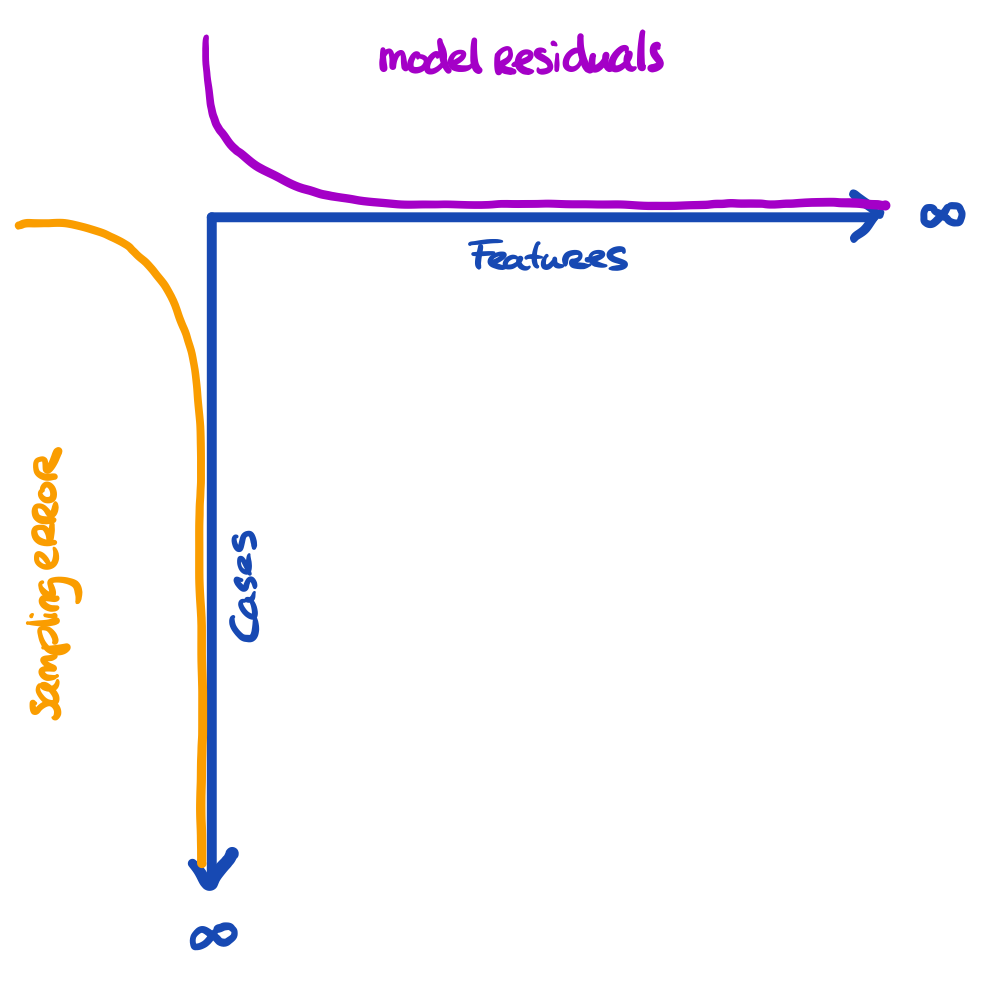
\includegraphics[width=0.9\textwidth,height=\textheight]{img/4. sidestep1.png}

\begin{itemize}
\item
  The problem is a bit larger
\item
  We have three entities at play, here:

  \begin{enumerate}
  \tightlist
  \item
    The truth we're interested in
  \item
    The proxy that we have (e.g.~sample)
  \item
    The model that we're running
  \end{enumerate}
\item
  The more features we use, the more we capture about the outcome for
  the cases in the data
\item
  The more cases we have, the more we approach the true information All
  these things are related to uncertainty. Our model can still yield
  biased results when fitted to \(\infty\) features. Our inference can
  still be wrong when obtained on \(\infty\) cases.
\end{itemize}
\end{frame}

\begin{frame}{Sidestep}
\protect\hypertarget{sidestep-1}{}
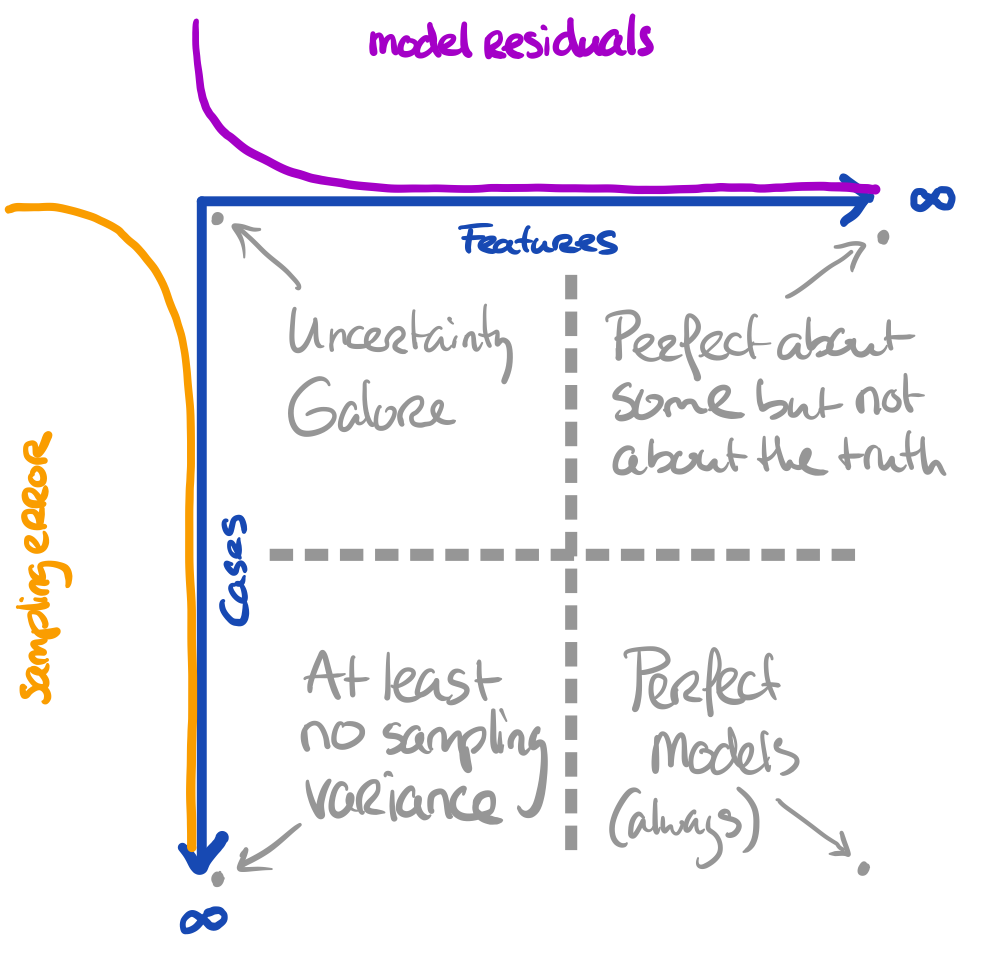
\includegraphics[width=0.9\textwidth,height=\textheight]{img/5. sidestep2.png}

\begin{itemize}
\item
  The problem is a bit larger
\item
  We have three entities at play, here:

  \begin{enumerate}
  \tightlist
  \item
    The truth we're interested in
  \item
    The proxy that we have (e.g.~sample)
  \item
    The model that we're running
  \end{enumerate}
\item
  The more features we use, the more we capture about the outcome for
  the cases in the data
\item
  The more cases we have, the more we approach the true information
\end{itemize}

\textbf{Core assumption: all observations are bonafide}
\end{frame}

\begin{frame}{Uncertainty simplified}
\protect\hypertarget{uncertainty-simplified}{}
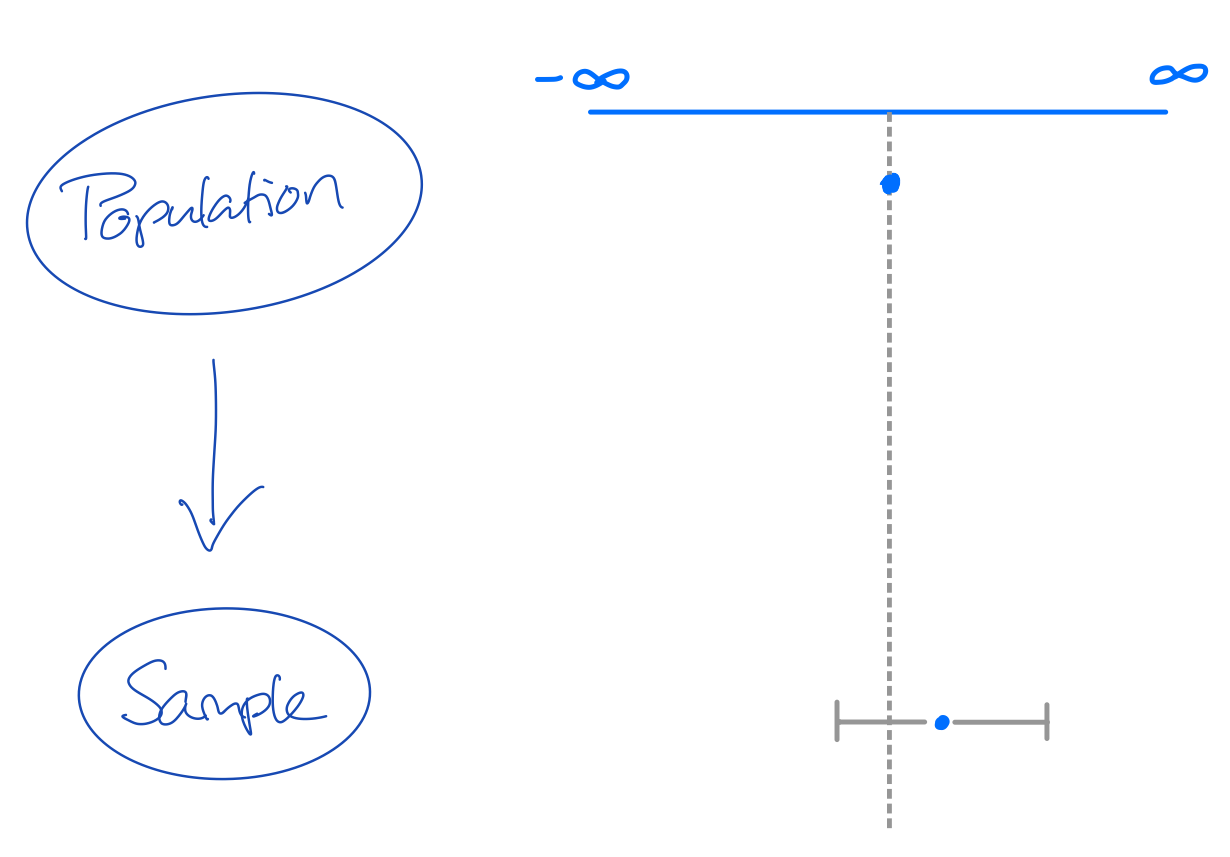
\includegraphics[width=0.9\textwidth,height=\textheight]{img/6. Sample_uncertainty.png}

When we do not have all information \ldots{}

\begin{enumerate}
\tightlist
\item
  We need to accept that we are probably wrong
\item
  We just have to quantify how wrong we are
\end{enumerate}

In some cases we estimate that we are only a bit wrong. In other cases
we estimate that we could be very wrong. This is the purpose of testing.
The uncertainty measures about our estimates can be used to create
intervals
\end{frame}

\begin{frame}{Confidence intervals}
\protect\hypertarget{confidence-intervals}{}
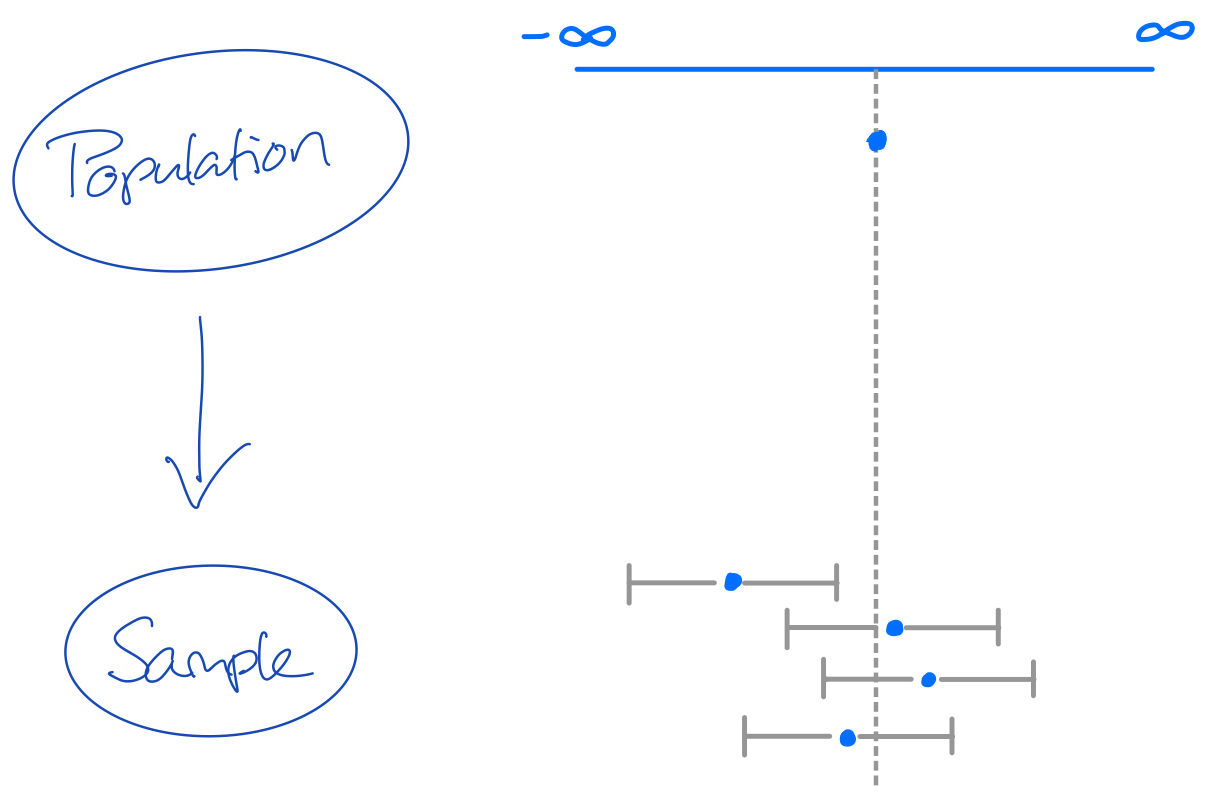
\includegraphics[width=0.9\textwidth,height=\textheight]{img/7. confidence_intervals.png}

Confidence intervals can be hugely informative!

If we sample 100 samples from a population, then a \emph{95\% CI} will
cover the population value at least 95 out of 100 times.

\begin{itemize}
\tightlist
\item
  If the coverage \textless95: bad estimation process with risk of
  errors and invalid inference
\item
  If the coverage \textgreater95: inefficient estimation process, but
  correct conclusions and valid inference. Lower statistical power.
\end{itemize}
\end{frame}

\begin{frame}{The other type of intervals}
\protect\hypertarget{the-other-type-of-intervals}{}
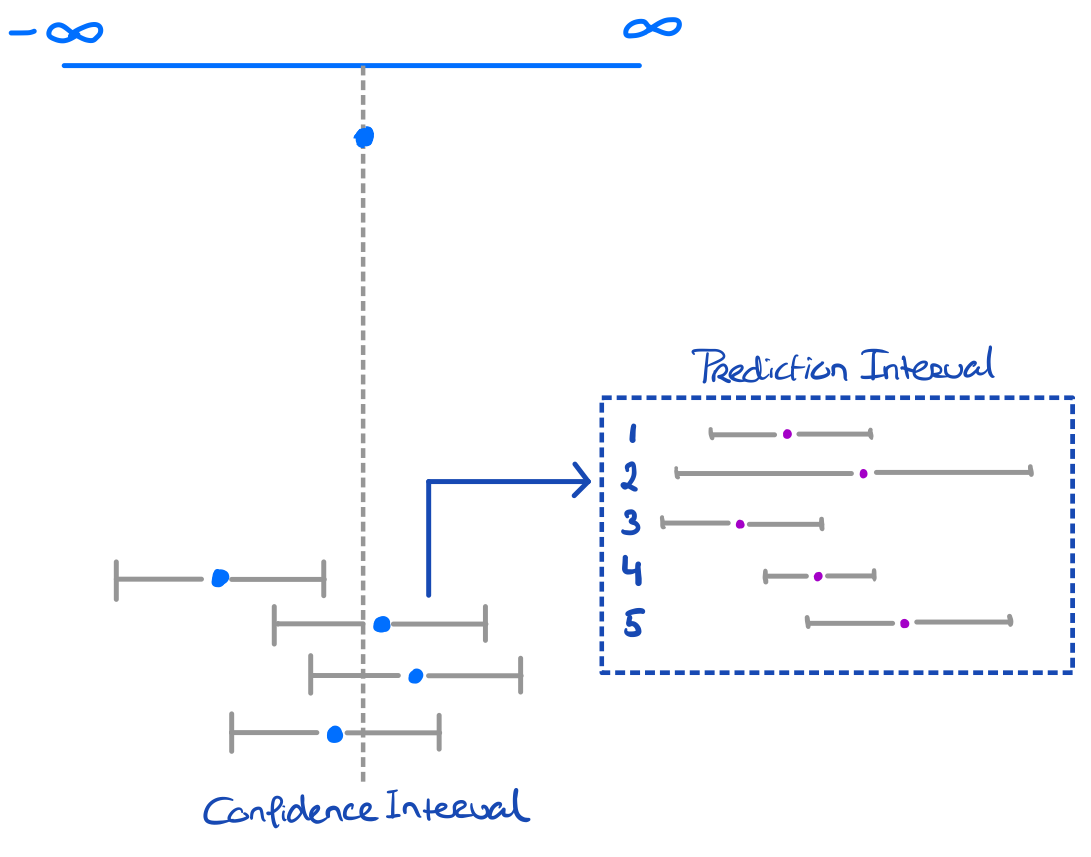
\includegraphics[width=0.9\textwidth,height=\textheight]{img/8. prediction_intervals.png}

Prediction intervals can also be hugely informative!

Prediction intervals are generally wider than confidence intervals

\begin{itemize}
\tightlist
\item
  This is because it covers inherent uncertainty in the data point on
  top of sampling uncertainty
\item
  Just like CIs, PIs will become more narrow (for locations) where more
  information is observed (less uncertainty)
\item
  Usually this is at the location of the mean of the predicted values.
\end{itemize}

\textbf{Narrower intervals mean less uncertainty. It does not mean less
bias!}
\end{frame}

\begin{frame}{The holy trinity}
\protect\hypertarget{the-holy-trinity}{}
Whenever I evaluate something, I tend to look at three things:

\begin{itemize}
\tightlist
\item
  bias (how far from the truth)
\item
  uncertainty/variance (how wide is my interval)
\item
  coverage (how often do I cover the truth with my interval)
\end{itemize}

As a function of model complexity in specific modeling efforts, these
components play a role in the bias/variance tradeoff

\includegraphics[width=0.4\textwidth,height=\textheight]{https://upload.wikimedia.org/wikipedia/commons/thumb/9/9f/Bias_and_variance_contributing_to_total_error.svg/2560px-Bias_and_variance_contributing_to_total_error.svg.png}
\end{frame}

\begin{frame}{Now with missingness}
\protect\hypertarget{now-with-missingness}{}
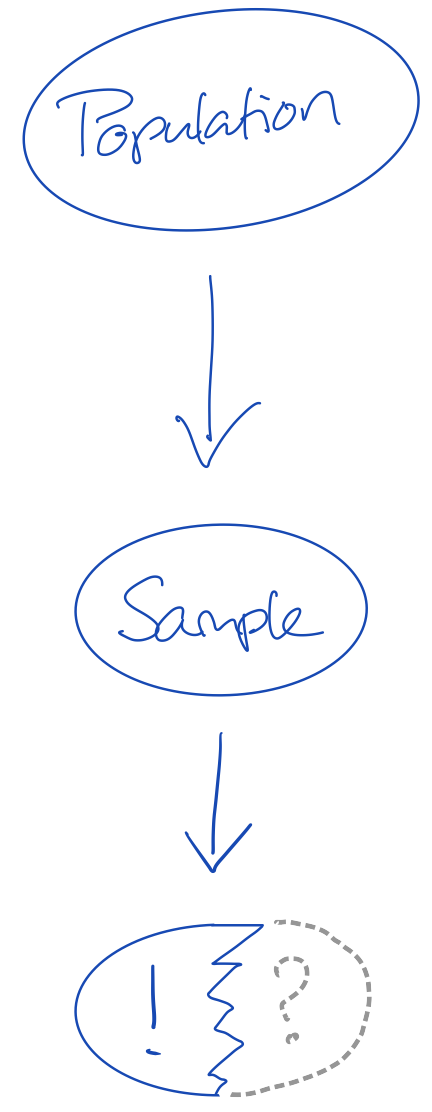
\includegraphics[width=0.6\textwidth,height=\textheight]{img/9.missingness.png}

We now have a new problem:

\begin{itemize}
\tightlist
\item
  we do not have the whole truth; but merely a sample of the truth
\item
  we do not even have the whole sample, but merely a sample of the
  sample of the truth.
\end{itemize}

Q4. What would be a simple solution to allowing for valid inferences on
the incomplete sample? Q5. Would that solution work in practice?
\end{frame}

\begin{frame}{Now with missingness}
\protect\hypertarget{now-with-missingness-1}{}
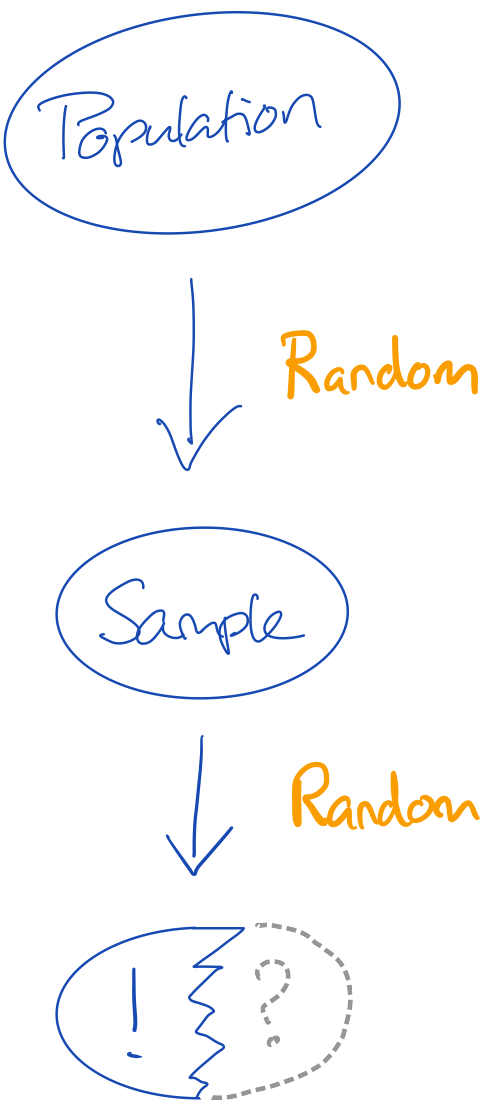
\includegraphics[width=0.68\textwidth,height=\textheight]{img/10. missingness_simplified.png}

We now have a new problem:

\begin{itemize}
\tightlist
\item
  we do not have the whole truth; but merely a sample of the truth
\item
  we do not even have the whole sample, but merely a sample of the
  sample of the truth.
\end{itemize}

Q4. What would be a simple solution to allowing for valid inferences on
the incomplete sample? Q5. Would that solution work in practice?
\end{frame}

\begin{frame}{Multiple imputation}
\protect\hypertarget{multiple-imputation}{}
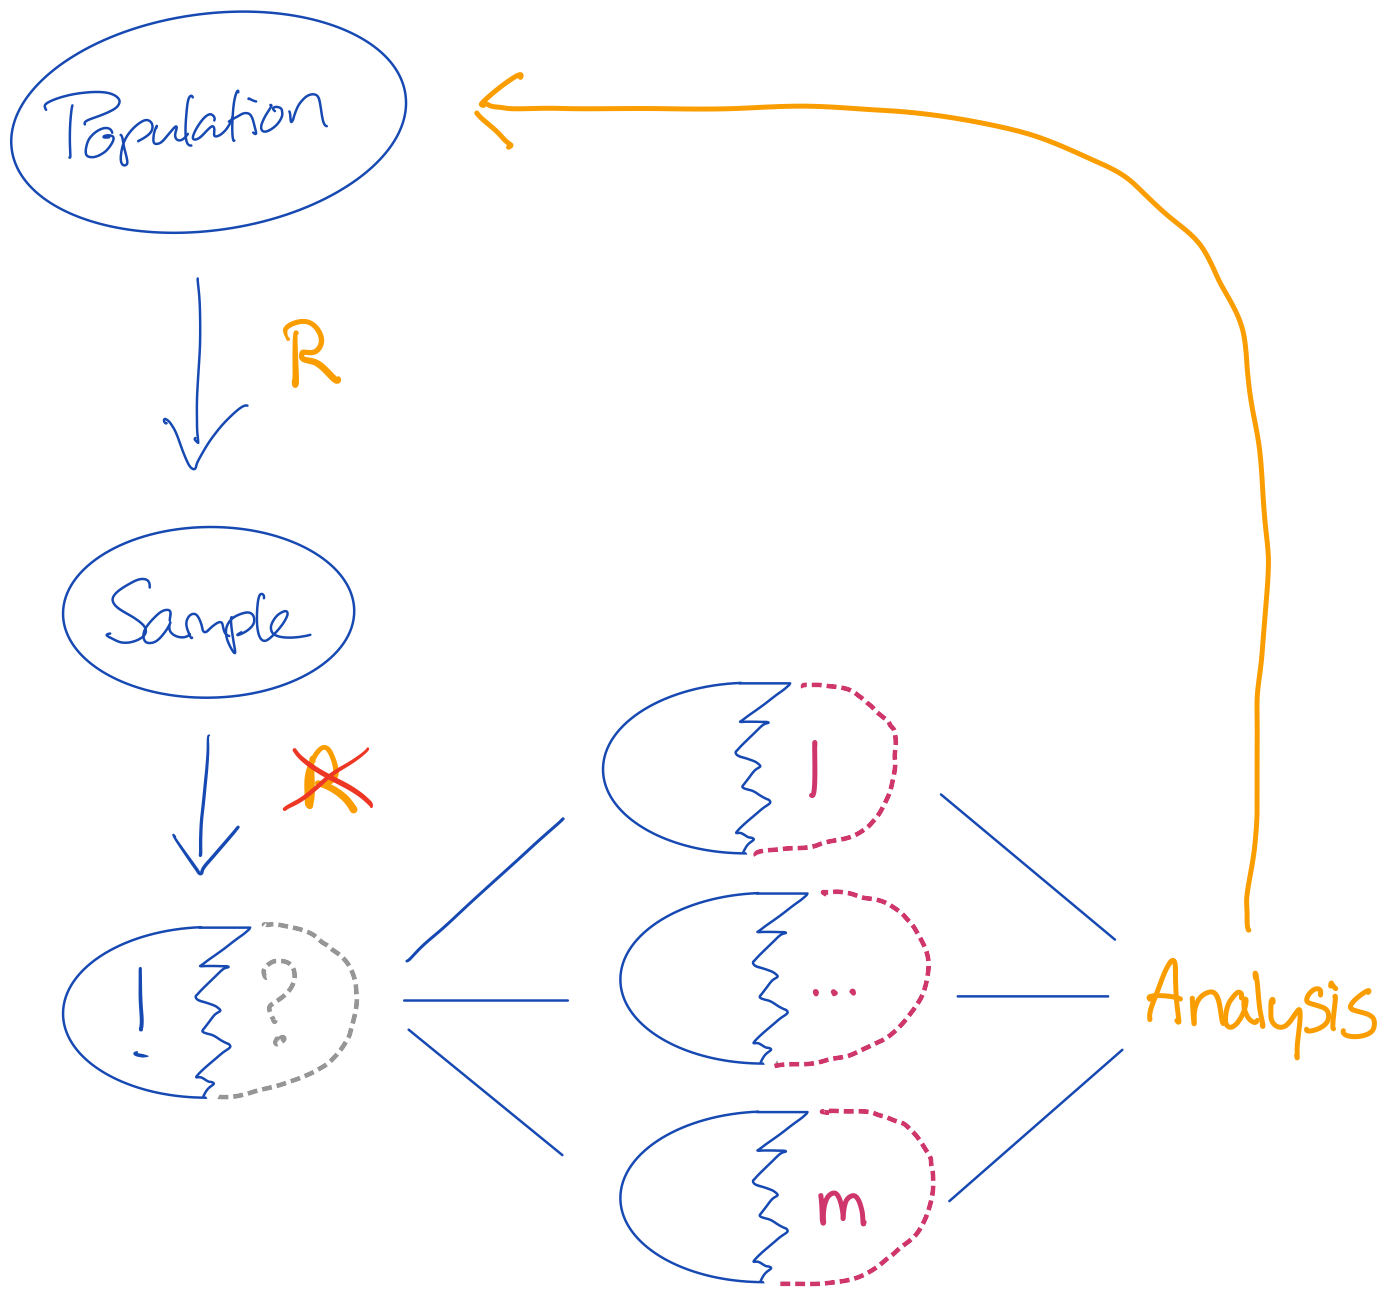
\includegraphics[width=0.8\textwidth,height=\textheight]{img/11. missingness_solved.png}

There are two sources of uncertainty that we need to cover:

\begin{enumerate}
\tightlist
\item
  \textbf{Uncertainty about the missing value}:when we don't know what
  the true observed value should be, we must create a distribution of
  values with proper variance (uncertainty).
\item
  \textbf{Uncertainty about the sampling}:nothing can guarantee that our
  sample is the one true sample. So it is reasonable to assume that the
  paramaters obtained on our sample are biased.
\end{enumerate}

\textbf{More challenging if the sample does not randomly come from the
population or if the feature set is too limited to solve for the
substantive model of interest}
\end{frame}

\begin{frame}{Now how do we know we did well?}
\protect\hypertarget{now-how-do-we-know-we-did-well}{}
I'm really sorry, but:

We don't. In practice we may often lack the necessary comparative
truths!

For example:

\begin{enumerate}
\tightlist
\item
  Predict a future response, but we only have the past
\item
  Analyzing incomplete data without a reference about the truth
\item
  Estimate the effect between two things that can never occur together
\item
  Mixing bonafide observations with bonafide non-observations
\end{enumerate}
\end{frame}



\end{document}
